% !TEX TS-program = pdflatex
% !TEX encoding = UTF-8 Unicode

% This is a simple template for a LaTeX document using the "article" class.
% See "book", "report", "letter" for other types of document.

\documentclass[11pt]{article} % use larger type; default would be 10pt

\usepackage[utf8]{inputenc} % set input encoding (not needed with XeLaTeX)
\usepackage[backend=biber, style=authoryear]{biblatex}

% basic bib file
\addbibresource{bibliography.bib}
% by lit type
\addbibresource{Literature/Past_Similar_Work/related_work.bib}
\addbibresource{Literature/Network_Analysis/network_lit.bib}
\addbibresource{Literature/Bicycling/general_cycling.bib}

%%% Examples of Article customizations
% These packages are optional, depending whether you want the features they provide.
% See the LaTeX Companion or other references for full information.

%%% PAGE DIMENSIONS
\usepackage{geometry} % to change the page dimensions
\geometry{a4paper} % or letterpaper (US) or a5paper or....
% \geometry{margin=2in} % for example, change the margins to 2 inches all round
% \geometry{landscape} % set up the page for landscape
%   read geometry.pdf for detailed page layout information

%\usepackage{graphicx} % support the \includegraphics command and options

\usepackage[parfill]{parskip} % Activate to begin paragraphs with an empty line rather than an indent

%%% PACKAGES
\usepackage{booktabs} % for much better looking tables
\usepackage{array} % for better arrays (eg matrices) in maths
\usepackage{paralist} % very flexible & customisable lists (eg. enumerate/itemize, etc.)
\usepackage{verbatim} % adds environment for commenting out blocks of text & for better verbatim
\usepackage{subfig} % make it possible to include more than one captioned figure/table in a single float
\usepackage{graphicx}
\usepackage{multirow} % allows multipel rows per cell
% These packages are all incorporated in the memoir class to one degree or another...

%%% HEADERS & FOOTERS
\usepackage{fancyhdr} % This should be set AFTER setting up the page geometry
\pagestyle{fancy} % options: empty , plain , fancy
\renewcommand{\headrulewidth}{0pt} % customise the layout...
\lhead{}\chead{}\rhead{}
\lfoot{}\cfoot{\thepage}\rfoot{}

%%% SECTION TITLE APPEARANCE
\usepackage{sectsty}
\allsectionsfont{\sffamily\mdseries\upshape} % (See the fntguide.pdf for font help)
% (This matches ConTeXt defaults)

%%% ToC (table of contents) APPEARANCE
\usepackage[nottoc,notlof,notlot]{tocbibind} % Put the bibliography in the ToC
\usepackage[titles,subfigure]{tocloft} % Alter the style of the Table of Contents
\renewcommand{\cftsecfont}{\rmfamily\mdseries\upshape}
\renewcommand{\cftsecpagefont}{\rmfamily\mdseries\upshape} % No bold!

%%% END Article customizations

%%% The "real" document content comes below...

\title{\vspace{-3.0cm}Review of Literature on Cycle Network Analysis}
\author{Author}
%\date{} % Activate to display a given date or no date (if empty),
         % otherwise the current date is printed 

\begin{document}
\maketitle


\section{Introduction}

Half of the world's population lives in cities. Cycling is of obvious importance to the well being of the world's  urban population in terms of the macro-climate crisis, local pollution problems, and public health issues. A commonly researched question is ``what factors have the most significant effect on cycling rates?'' The review of literature that follows will argue that the majority of work on this question approaches the matter from a perspective of discrete policy intervention and the effect of marginal improvements on cycling. This fails to build a comprehensive theory of cycling rates that a network analysis approach can offer. Only network theory can offer a high level look at the level of service in a community. The review that follows takes the structure of an initial look at typical literature considering how to promote cycling, recent attempts to use network analysis to accomplish this same goal, and closes with a look at work in network analysis that can inform applying the field to cycle networks. The overarching theme of the review and the research that is proposed is the idea that no individual intervention is sufficient to change behavior until a comprehensive network of infrastructure that reflects the importance of locations according to centrality is created. The implication of this view is that infrastructure changes are unlikely to have a meaningful effect on behavior in the system until a critical mass or tipping point is reached. 
%%%%%%%%%%%%%%%%%%%%%%%%%%%%%%%%%%%%%%%%%%%%%%%%%%%%%%%%%%%%%%%%%%%%%%%%%%%%%%%%%%%%%%%%%%%%%%%%%%%%%%%%%%%%%%%%%%

\section{Literature Review}

\subsection{Relevant Literature regarding cycling generally}

Dill, 4 types of cyclists, ``strong and fearless'', ``enthused and confident'', ``interested but concerned'', no way no how''.   \cite{dill2013four}

Ellett, State Paranoia and urban Cycling: fear is a significant factor during an urban cycling trip. \cite{ellett2018state}

Fajans, Why Bicyclists Hate Stop Signs, built environment has a meaningful impact on the energy required for a journey by bicycle. \cite{fajans2001bicyclists}

Gosse, Estimating Spatially and Temporally continuous bicycle volumes by using sparse data. Difficult to get an estimate of bike traffic with the data available. \cite{gosse2014estimating}

Gu, The cost effectiveness of bike lanes in New York City, ROI is high for bike lanes. \cite{gu2017cost}

Heinen, Commuting by bicycle, an overview of the lit: investigates the determinants for commuting by bicycle. \cite{heinen2010commuting}

Kondo: Where do bike lanes work best a Bayesian spatial model of bicycle lanes and bicycle crashes. Bike lanes have different values in different places. \cite{kondo2018bike}

Li, Physical environments influencing bicyclists' perception of comfort on separated and on-street bicycle facilities. Simple look at perceived safety in different cycling environments. \cite{li2012physical}

Parkin, Models of perceived cycling risk and route acceptability. The factors that influence perceived safety \cite{parkin2007models}

Savan, Integrated Strategies to accelerate the adoption of cycling for transportation, Psychological behavioral change approach to increasing cycling. \cite{savan2017integrated}

Stinson, Route preferences of experienced and inexperienced bicycle commuters. Different types of cyclists react differently to traffic stress. \cite{stinson2005comparison}

Thigpen, States of change approach to explore opportunities for increased bicycle commuting. Focuses on changing cyclists rather than infrastructure. \cite{thigpen2015using}

Vandenbulcke, Predicting cycling accident risk in Brussels: A Spatial case control approach. The things cyclists perceive as dangerous are dangerous. \cite{vandenbulcke2014predicting}

%%%%%%%%%%%%%%%%%%%%%%%%%%%%%%%%%%%%%%%%%%%%%%%%%%%%%%%%%%%%%%%%%%%%%%%%%%%%%%%%%%%%%%%%%%%%%%%%%%%%%%%%%%%%%%%%%%

\subsection{Literature addressing cycling From a network perspective}

Akbarzadeh, Designing Bike networks using the concept of network clusters, Taxi trips to indicate links between nodes. Not a very good method for understanding where to build networks, needlessly complicated. \cite{akbarzadeh2018designing}


Data from online survey to get a cost function, predicted travel routes, compared to shortest route, which is used to measure network connectivity. 
%%%%%%%%%%%%%%%%%%%%%

\textbf{
Counter intuitively, if one was to measure the total distance of the network, that would incentivize less direct links, since these tend to be longer.}  
%%%%%%%%%%%%%%%%%%%%%%
\cite{boisjoly2019bicycle} 



Buehler \& Dill's  particularly helpful review of literature on bike networks uses a framework that groups the literature by two categories, that focusing on the links of the network, different types of cycle lanes, and that focusing on the nodes of the network, intersections. It ends by addressing the possibility of a cohesive study of a bicycle network holistically.

	For instance \textit{One study linked cycling levels to self reported measures of the bicycling environment, including being able to take shortcuts on a bicycle compared to routes available to cars. This measure of connectivity was found to be significant (Titze, Stronegger, Janschitz, \& Oja, 2008).}
	
	\textit{ a recent paper using aggregate bicycle commuting data from 74 US cities (Schoner \& Levinson, 2014). The authors develop several different measures that represent the size, connectivity, density, fragmentation, and directness of the bicycle network. The density of the bikeway network (all types of facilities combined) had the largest elasticity value, larger than connectivity, fragmentation, and directness combined.}
	
	This includes a Bicycle Compatibility Index (BCI) combination of distance and safety, Bicycle level of service (BLOS) from ``Highway Capacity Manual'', \cite{Lowry} and Level of Traffic Stress (LTS) \cite{Mekuria and Furth} a four point scale based on architectural features of the route.
	
	Basically, these four don't really constitute a holistic approach still. 
	
	Difficulty of validating the effect because there isn't a lot of cyclist behavior data available.
	
	
Since Buehler's literature review was published 115 subsequent papers have cited it but only a few have taken the author's central recommendation that a holistic approach to evaluating a bike network be employed. 


Starting point for the lit review since it covers everthing prior to 2016, node, link and network focused lit. 
\cite{buehler2016bikeway}

Edmonton did a rapid full network implementation instead of a incremental approach. 
\cite{cabral2019low}

Genetic algorithm used to solve a mathematical program with equillibrium constraints. 
\cite{doorley2019designing}

Optimization problem: retrofitting existing roadway infrastructure for bicycles. Minimize cost while conncting all origin destination pairs considering bicycling level of service. 
\cite{duthie2014optimization}

San Jose, vizualizing and analyzing lack of connectivity. 
First low stress network analysis. Focuses on \% of pairs connected with low stress links. A few improvements would dramatically increase connectivity. 
\cite{furth2016network}

Seattle , tool for analyzing low stress connectivity. 
\cite{lowry2016prioritizing}

Compare connectivity for different types of cyclists in different neighborhoods. 
\cite{lowry2017quantifying}

Algorithm for bicycle netowrk design: balance interests of users and planners, construction v user cost, proportional to distance, adjusted for usage rates, and ``discontinuities'' 
\cite{mauttone2017bicycle}

Original study on low stress network connectivity
\cite{mekuria2012low}

%\cite{macmillan2017understanding}

Algo for bike network design, filter out ``ineligible streets'' then balance between improvement for cyclists and cost for drivers, then optimize with genetic algorithm, 
\cite{mesbah2012bilevel}

%\cite{milakis2012planning}

Predicti bike kilometers traveled with network indicators, land use and road facility. Vancouver Canada. Bayesian model with spatial random effects. 
\cite{osama2017models}


Does level of traffic stress explain bicycle travel behavior. Uses census data , mode choice data, and regional household survey data to test relatinoship between traffic stress and bicycle travel behavior. Questions LTS. 
\cite{wang2016does}


%%%%%%%%%%%%%%%%%%%%%%%%%%%%%%%%%%%%%%%%%%%%%%%%%%%%%%%%%%%%%%%%%%%%%%%%%%%%%%%%%%%%%%%%%%%%%%%%%%%%%%%%%%%%%%%%%%


\subsection{Network analysis Literature relevant to the research methodology proposed}
\textbf{
The key questions that need to be addressed by this lit are: 
\begin{itemize}
\item How to rigorously compare distributions of centrality
\item Dual or Primal graph? 
\item How to actually do what I intend to do, a manual of some sort?
\item Anything to do with growing one network on top of another. 
\item Address and dismiss multiplex  networks approach. 
\item The potential for a ``transition''
\item Which centrality networks to use?
\item Justify centrality as a way of prioritizing connectivity as a shortcut
\item Potential for local communities of small world world networks? 
\item Can planar graphs be small world?
\item Community identification in planar graphs? 
\item Could a weighted random walk be a good proxy for trips? 
\end{itemize}
}


Crossover from scale free to spatial network:

What is distinct about spatial networks: distance weighted, preferntial attachment and distance selection. When distance effect is significant, connectivity dist has a cutoff depending on node density, clustering coeff is very high, assortivity, positive max to degree correlation
\cite{barthelemy2003crossover}

Spatial Networks:

relevant part is the review of processes that take place on spatial networks. 
Phase transitions, random walks, synchronization, navigation, resilience, disease spread. 
\cite{barthelemy2011spatial}

Centrality Measures in spatial networks of urban streets

Uses 4 indices of centrality: closeness, betweenness, straightness, information. 
\cite{crucitti2006centrality}


Nonparametric resampling of random walks for spectral network clustering

goal is to assess the statistical significance of clustering and robustness of community identification. 
\cite{fallani2014nonparametric}


\cite{feliciotti2016design}

\cite{}

\cite{}

\cite{}

\cite{}

\cite{}

Planar graphs
Connection between centrality and economic activity
	Porta 2012, Barcelona
Transitions in spatial networks: percolation and small world stuff
Multiplex networks probably not relevant because it's hard to take a bike on a train or bus or whatever
	Urban accessibility measurement
		Porta 
		Biazzo
		Need to weight edges but inverse of distance



%%%%%%%%%%%%%%%%%%%%%%%%%%%%%%%%%%%%%%%%%%%%%%%%%%%%%%%%%%%%%%%%%%%%%%%%%%%%%%%%%%%%%%%%%%%%%%%%%%%%%%%%%%%%%%%%%%

\section{Intended research Questions and Methodology}


Possible Research Questions
	Conservative: What does London look like to a cyclist? Build network according to different rules and compare
		traffic stress
			intersections
			streets
		no right turns
		only official bike network
			
	Moderate: community detection using the stuff from the conservative project, where is the network the strongest?
	Aggressive: how closely has the London network followed an optimal growth of network on network? 
		This could use standard measures of street centrality for the road network and look at accessibility for the most important streets. 
		Or compare centrality distribution of bike networks to streets, use street centrality for given bike lane, are lanes relatively central or no? 
		Or compare evolution of rd networks to evolution of bike networks
		
Straightness is an interesting one but distance matters most I guess. 
Congestion is not really a problem for cyclists

Road network
	attach attributes to links and nodes
		bike lane with type
		traffic characteristics
		road characteristics
		traffic incidents
		
Remove links and nodes according to attributes

Compare distribution of centrality between estimated bike network and real road network. 

Use Cycle Hire data to validate centrality preference?
	But hires are station to station so would have to show that the probability of a station being a destination for a trip is influenced by stations centrality. 

Steps:

	get london road network
		just the data
		get the distribution of centrality measures
	get the london bike network
		just the data
		get the distribution of centrality measures
		
	give a road an index grade
		using accident stats and road characteristics
		
	add ``safe'' roads to cycle network
	
	compare disributions of centrality scores between road network and bike network. 
	
	compare network before and after Super Highway constructions

%%%%%%%%%%%%%%%%%%%%%%%%%%%%%%%%%%%%%%%%%%%%%%%%%%%%%%%%%%%%%%%%%%%%%%%%%%%%%%%%%%%%%%%%%%%%%%%%%%%%%%%%%%%%%%%%%%

\section{}

\section{}

%%%%%%%%%%%%%%%%%%%%%%%%%%%%%%%%%%%%%%%%%%%%%%%%%%%%%%%%%%%%%%%%%%%%%%%%%%%%%%%%%%%%%%%%%%%%%%%%%%%%%%%%%%%%
 
%\begin{itemize}
%\item one
%\item two
%  \begin{itemize}
%  \item one point one
%  \item one point two
%  \end{itemize}
%\end{itemize}
%
%\subsection{Subsection 1}
%
%\begin{figure}
%\centering
%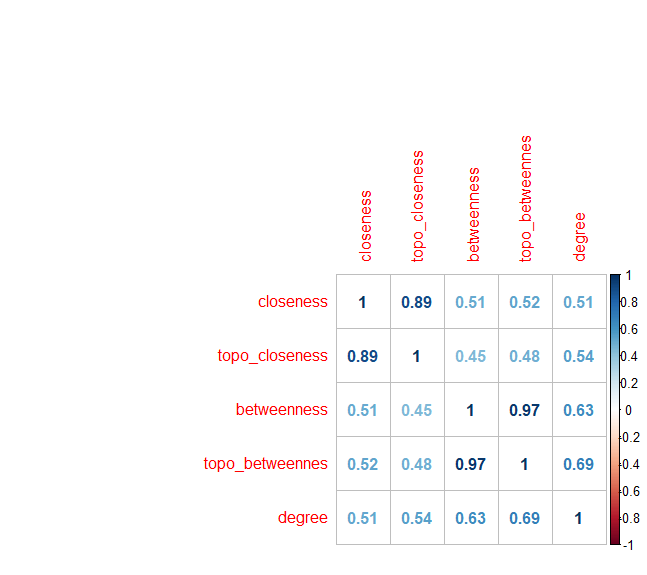
\includegraphics[width=0.8\textwidth]{example}
%\caption{Correlation between station/node metrics}
%\end{figure}
%
%\begin{tabular}{|l|l|l|l|}\hline
%  \multirow{10}{*}{numeric literals} 				& \multirow{5}{*}{integers} 	& in decimal 					& \verb|8743| \\ \cline{3-4}
%  					    				& 				       	& \multirow{2}{*}{in octal}   		& \verb|0o7464| \\ \cline{4-4}
%  					    				& 					& 						& \verb|0O103| \\ \cline{3-4}
%  					    				& 					& \multirow{2}{*}{in hexadecimal}	& \verb|0x5A0FF| \\ \cline{4-4}
% 				 	    				& 					& 						& \verb|0xE0F2| \\ \cline{2-4}
%  					    				& \multirow{5}{*}{fractionals} 	& \multirow{5}{*}{in decimal} 		& \verb|140.58| \\ \cline{4-4}
% 				 					& 					& 						& \verb|8.04e7| \\ \cline{4-4}
%  									& 					& 						& \verb|0.347E+12| \\ \cline{4-4}
%  									& 					& 						& \verb|5.47E-12| \\ \cline{4-4}
%  									& 					& 						& \verb|47e22| \\ \cline{1-4}
%  \multicolumn{3}{|l|}{\multirow{3}{*}{char literals}} 													& \verb|'H'| \\ \cline{4-4}
%  \multicolumn{3}{|l|}{} 																	& \verb|'\n'| \\ \cline{4-4}          %% here
%  \multicolumn{3}{|l|}{} 																	& \verb|'\x65'| \\ \cline{1-4}        %% here
%  \multicolumn{3}{|l|}{\multirow{2}{*}{string literals}} 												& \verb|"bom dia"| \\ \cline{4-4}
%  \multicolumn{3}{|l|}{} 																	& \verb|"ouro preto\nmg"| \\ \cline{1-4}          %% here
%\end{tabular}
%
%\begin{verbatim}
%use pseudocode
%\end{verbatim}
%
%\textit{italics}
%\textbf{bold}

XXXX words excluding headings, figures, and references. \\

\nocite{*}

\medskip


\printbibliography


\end{document}
